\documentclass[11pt]{article}

\usepackage[a4paper,margin=1.05in]{geometry}
\usepackage{mathpazo}
\usepackage[T1]{fontenc}
\usepackage{amsmath,amssymb}
\usepackage{microtype}
\usepackage{booktabs}
\usepackage{tabularx}
\usepackage{enumitem}
\usepackage{parskip}
\usepackage{titlesec}
\usepackage{fancyhdr}
\usepackage{tikz}
\usepackage{tcolorbox}
\usepackage[colorlinks=true,linkcolor=accent,urlcolor=accent,citecolor=accent]{hyperref}

\usetikzlibrary{arrows.meta,positioning,fit,backgrounds,calc}
\tcbuselibrary{skins,breakable}

%% ---------------------------------------------------------------- palette
\definecolor{accent}{HTML}{1F5C6B}      % deep slate-teal -- structure
\definecolor{accentbg}{HTML}{DCE9EC}
\definecolor{softgray}{HTML}{6B6B6B}
\definecolor{vocabc}{HTML}{8A3F5F}      % first-use vocabulary
\definecolor{warnrule}{HTML}{B8860B}
\definecolor{warnbg}{HTML}{FBF0D9}

%% First-use vocabulary is a distinct visual channel from ordinary emphasis.
\newcommand{\vocab}[1]{\textcolor{vocabc}{\textbf{#1}}}

%% ---------------------------------------------------------------- styling
\titleformat{\section}{\large\bfseries\color{accent}}{\thesection}{0.7em}{}
\titleformat{\subsection}{\normalsize\bfseries}{\thesubsection}{0.6em}{}
\setlist[itemize]{leftmargin=1.3em,itemsep=2pt,topsep=3pt}

\pagestyle{fancy}
\fancyhf{}
\renewcommand{\headrulewidth}{0.3pt}
\lhead{\small\color{softgray}qsp-inference · The statistical model}
\rhead{\small\color{softgray}\thepage}

\newtcolorbox{keybox}{
  enhanced, breakable, colback=accentbg!55, colframe=accent,
  boxrule=0pt, leftrule=2.5pt, arc=1pt, left=10pt, right=10pt, top=8pt, bottom=8pt
}

\newtcolorbox{hardbox}[1]{
  enhanced, breakable, colback=warnbg, colframe=warnrule,
  boxrule=0pt, leftrule=2.5pt, arc=1pt, left=10pt, right=10pt, top=7pt, bottom=7pt,
  title={\bfseries #1}, coltitle=warnrule, fonttitle=\bfseries,
  attach title to upper={\par\medskip}, colbacktitle=warnbg
}

\renewcommand{\th}{\theta}
\newcommand{\xobs}{x_{\mathrm{obs}}}

%% ================================================================ document
\begin{document}

\begin{center}
  {\LARGE\bfseries\color{accent} The Statistical Model}\\[5pt]
  {\large\color{accent}\texttt{qsp-inference}}\\[12pt]
  {\small One probability model, two questions: the single-patient posterior}\\
  {\small and the virtual population}\\[10pt]
  {\color{softgray}\rule{0.35\textwidth}{0.4pt}}
\end{center}

\vspace{0.6em}

\noindent\emph{The section to read first. It sets down the probability model that the
rest of the package implements, and the two questions we ask of it --- no code, no
\texttt{Stage 1 / Stage 2}, no jargon left undefined. Terms are given three names where
they have three: one from Bayesian statistics, one from pharmacometrics, one from the
simulation-based-inference literature, so that whichever field you arrived from, you can
see the object is one you already know.}

\vspace{0.8em}

\section{The setup}

A mechanistic model of this kind carries a few hundred parameters --- rate constants,
half-saturation concentrations, homeostatic cell densities --- and almost none of them
can be measured in the clinical setting the model is meant to describe. The usual
practice is to take a literature point value for each and attach a range wide enough to
look cautious. That yields parameterizations that run, but it answers no question about
how much the data actually constrain, and it cannot tell you when a calibration target
is simply out of the model's reach.

We take the other route: write the model down as a probability model, and infer. One
question runs underneath everything that follows, and it is worth stating plainly before
the notation arrives.

\begin{keybox}
If we trust the mechanism, and we trust the priors, then the calibration should fit the
data on its own --- whether the target is a single median patient or an entire
population. Where it does, there is nothing left to hand-tune. Where it does not, the
failure is telling us something, and the job is to say precisely \emph{what kind} of
failure it is.
\end{keybox}

Most of the machinery here exists to turn that question from a slogan into something you
can actually answer.

\section{The generative model}

There is one model, and it has three pieces: a parameter vector, a prior over it, and a
rule for how parameters produce data.
\[
  \th \sim \pi(\th), \qquad x \mid \th \sim p(x \mid \th), \qquad \mathbb{E}[x \mid \th] = g(\th).
\]
The parameters $\th \in \mathbb{R}^d$ live on a log scale wherever they are positive
rates, so a prior is lognormal and the natural notion of distance between two values is
a ratio, not a difference. The prior $\pi(\th)$ is informative and built from external
data; the next section is about how. The map $g(\th)$ is the mechanism itself ---
integrate the ODE system forward and reduce each trajectory to the quantity that was
measured --- and it is deterministic: a given $\th$ always produces the same $g(\th)$.

The randomness is the measurement, and it is deliberately \emph{not} assumed Gaussian.
For each observable the noise is taken from the observed statistic's own bootstrap
sampling distribution --- its skew, its tails, its bounds --- and convolved onto the
prediction, multiplicatively where the quantity is positive so that positivity is
preserved. Only when a target supplies no bootstrap does a parametric fallback step in,
and even then it is a lognormal or a Gaussian chosen \emph{per observable} by the
asymmetry of the reported confidence interval, not a blanket Normal. In the default path
there is no parametric noise family at all: the observation layer is itself available
only as a sampler.

The one feature that shapes every method downstream is that the likelihood
$p(x \mid \th)$ can be neither written down nor evaluated, for two compounding reasons:
the mean map $g$ is an ODE solve with no analytic form, and the noise layer, in its
default, is an empirical resampler rather than a density. We can \emph{draw} pairs
$(\th, x)$ as fast as we can simulate, but we cannot \emph{evaluate} the density of one.
Inference that needs only sampling --- not evaluation --- is called
\vocab{simulation-based} (equivalently, \emph{likelihood-free}): we learn the posterior
with a neural density estimator trained on simulations, and the observation noise enters
as augmentation on those training pairs, not as a likelihood we compute.

\begin{figure}[h]
\centering
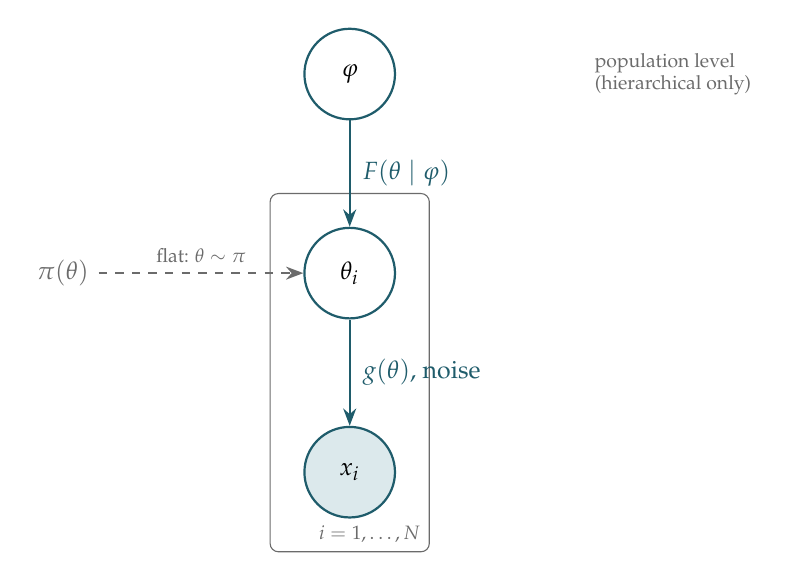
\begin{tikzpicture}[font=\small,
    latent/.style={circle,draw=accent,thick,minimum size=1.15cm,inner sep=1pt,fill=white},
    obs/.style={circle,draw=accent,thick,minimum size=1.15cm,inner sep=1pt,fill=accentbg},
    plate/.style={rectangle,draw=softgray,rounded corners=3pt,inner sep=12pt},
    flow/.style={-{Stealth[length=2.2mm]},accent,line width=0.8pt}]

  \node[latent] (phi) {$\varphi$};
  \node[latent,below=1.35cm of phi] (theta) {$\th_i$};
  \node[obs,below=1.35cm of theta] (x) {$x_i$};
  \node[left=2.6cm of theta,softgray] (pi) {$\pi(\th)$};

  \draw[flow] (phi) -- (theta) node[midway,right=1pt]{$F(\th\mid\varphi)$};
  \draw[flow] (theta) -- (x) node[midway,right=1pt]{$g(\th)$, noise};
  \draw[flow,dashed,softgray] (pi) -- (theta)
        node[midway,above,font=\scriptsize]{flat: $\th\sim\pi$};

  \node[right=2.4cm of phi,align=left,softgray,font=\scriptsize] {population level\\(hierarchical only)};

  \begin{scope}[on background layer]
    \node[plate,fit=(theta)(x)] (pl) {};
  \end{scope}
  \node[softgray,font=\scriptsize,anchor=south east] at (pl.south east) {$i=1,\dots,N$};
\end{tikzpicture}
\caption*{\small Cover the top node and it is the \emph{flat} model, $\th\sim\pi$,
$x\mid\th$. Include it and it is the \emph{population} model: a shared $\varphi$
generates each patient's $\th_i$.}
\end{figure}

\section{Two questions, one model}

The distinction between calibrating to a median patient and generating a virtual
population is not a distinction between two workflows. It is two questions asked of the
single model above, and it is the same distinction a mixed-effects modeler draws between
a typical-value fit and a random-effects distribution.

The first question fixes one observed summary $\xobs$ --- the target medians --- and asks
for the posterior $p(\th \mid \xobs)$. This is calibration in the ordinary sense: one set
of parameters, uncertainty and all, consistent with one observation. Call it the
\vocab{flat}, or single-unit, or fixed-effects problem.

The second question does not treat the parameters as fixed across patients. It supposes
each patient $i$ has their own $\th_i$, drawn from a population distribution
$F(\th \mid \varphi)$ with hyperparameters $\varphi = (\mu, \omega)$ --- a location and a
spread --- and the data are now summaries \emph{across a cohort}: a median and an
inter-quartile range for each target, over some real number of patients $n_j$. What we
infer is $\varphi$, and the \vocab{virtual population} is the fitted distribution
$F(\th \mid \hat\varphi)$. A virtual patient is a draw from it. That is all a virtual
patient is --- a sample from an estimated random-effects distribution --- and saying so
is the whole point of writing the model this way.

\begin{center}
\small
\begin{tabularx}{\textwidth}{@{}l X X@{}}
\toprule
 & \textbf{flat inference} & \textbf{virtual population} \\
\midrule
in Bayesian terms & single-unit posterior $p(\th\mid\xobs)$ & hierarchical model; infer $\varphi=(\mu,\omega)$ \\
in NLME terms & typical-value fit & the random-effects distribution ($\Theta$, $\Omega$) \\
the answer is & a posterior over $\th$ & a distribution $F(\th\mid\hat\varphi)$ over patients \\
a ``patient'' is & a posterior draw & a draw $\th\sim F(\th\mid\hat\varphi)$ \\
the data are & target medians & target (median, IQR) across $n_j$ patients \\
\bottomrule
\end{tabularx}
\end{center}

Nothing about the mechanism $g$, the prior $\pi$, or the observation model changes
between the two. Only the question does. The package is arranged around that fact: the
same simulator and the same prior serve both, and the population problem is the flat
problem with a level added on top.

\section{The prior is a measurement model, not a guess}

For a model this over-parameterized the prior is not a nuisance to be set wide and
forgotten. As the next section makes precise, the data identify only a handful of
directions in parameter space; along the rest, \emph{the prior is the answer the
calibration returns}. A prior that carries the answer for two hundred parameters has to
be built with the care one would give a likelihood.

So it is built, not asserted. Each quantitative claim in the literature is paired with a
small forward model that predicts \emph{that measurement} from a few parameters, and the
pair is inverted --- an ordinary measurement-error model. Three features are worth naming,
because each corresponds to a standard statistical device.

A source measured in the wrong context should count for less. Each source carries a
\vocab{translation sigma} that inflates its likelihood variance according to how far its
setting --- species, indication, assay --- sits from the one being modeled. This is the
between-study heterogeneity of a \vocab{random-effects meta-analysis}, the $\tau^2$ that
lets mouse data inform a human parameter without pretending to be human data.

It is also, exactly, a \vocab{power prior} (Ibrahim \& Chen 2000) --- the standard device
for borrowing strength from historical data under a discount. A power prior raises a
historical dataset's likelihood to a fractional power,
$\pi(\th \mid D_0, a_0) \propto L(\th \mid D_0)^{a_0}\,\pi_0(\th)$, and for a Gaussian
likelihood that is \emph{identical} to inflating the variance:
\[
  L^{a} \propto \exp\!\Big(-\tfrac{a\,(y - g(\th))^2}{2\sigma^2}\Big)
       = \text{kernel of } \mathcal{N}\big(y;\, g(\th),\ \sigma^2/a\big).
\]
So discounting a source by inflating its $\sigma$ \emph{is} discounting its likelihood by
an exponent $a_j = \sigma_j^2 / \tilde\sigma_j^2$; the two constructions coincide here
and diverge only for non-Gaussian likelihoods. Worth stating plainly because it locates
the relevance rubric in a literature with its own machinery: the rubric is a
\textbf{fixed, hand-specified} choice of those exponents, while the \emph{normalized}
power prior treats $a_0$ as random and infers it from how consistent a source turns out
to be with the others. That is the natural route to retiring the rubric as a manual
surface, and it is affordable exactly here --- Stage~1 chunks are small and already
sampled with NUTS, so the normalizing constant that makes inferred $a_0$ expensive is
within reach.

Parameters informed by the same measurement are correlated, and discarding that would
overstate what we know. The per-parameter marginals are therefore joined by a
\vocab{Gaussian copula} --- Sklar's construction, marginals for the uncertainty and a
correlation matrix for the dependence --- giving a genuine joint distribution that can be
both sampled and evaluated.

A parameter with no data of its own, but a mechanistic tie to one that does, enters as a
log-linear-Gaussian \vocab{derived} child of its anchor: it inherits the parent's width
and correlation instead of receiving an invented target of its own.

\section{Inference without a likelihood}

Since the likelihood can only be sampled, we estimate the posterior directly. Simulate
many pairs $(\th, x)$ from the model, fit a normalizing-flow conditional density
$q(\th \mid x)$ to them, and read it at $x = \xobs$. This is \vocab{neural posterior
estimation} (NPE), the amortized member of the simulation-based-inference family: the
cost is paid once, at training, after which any observation can be conditioned on
cheaply.

Three refinements matter, and each is a named technique rather than a tuning knob. The
distribution we \emph{draw training samples from} need not be the prior we \emph{report
under}. We draw from a wider \vocab{proposal} $\tilde\pi$, wide in the directions the data
can actually inform, where coverage is worth paying for, and recover the posterior under
the anchored prior $\pi$ by self-normalized importance weighting, $w \propto
\pi/\tilde\pi$, watching the effective sample size. Separating the two is what lets the
proposal be a computational choice and the prior a scientific one. Left to itself the
proposal is still an ad hoc width; \vocab{truncated sequential NPE} (Deistler et al.\
2022) removes that by narrowing it, round by round, toward the region the posterior
occupies, which also keeps the importance weights well behaved. The result reported is
the posterior under $\pi$; the proposal has done its work and drops out.

\section{Populations: the level on top}

The population problem adds the hierarchy the flat problem omits. Patient $i$ draws
$\th_i \sim F(\th \mid \varphi)$, the hyperparameter $\varphi = (\mu, \omega)$ has its own
hyperprior, and the observations are cohort summaries. We infer
$p(\varphi \mid \text{summaries})$ by amortized inference over simulated cohorts, and emit
the virtual population as draws at $\hat\varphi$.

Two choices here are statistical rather than incidental. First: you cannot estimate two
hundred population spreads when only a few directions carry signal, so $\log\omega$ is
inferred along the leading eigen-directions of $\pi$'s covariance --- the directions the
data speak to --- and left at its anchored prior value everywhere else. The
identifiability limit that governs the flat posterior governs the population spread in
exactly the same way, and the eigenbasis is where that limit is imposed. Second: the
amount a target says about the spread should match how many patients it was measured in.
A target reported over six patients constrains $\omega$ weakly; one over nine hundred
constrains it tightly. Cohort summaries are drawn at each target's real published $n$, so
the evidence is weighted honestly.

An older construction --- generate a cloud of plausible patients and reweight it to match
the observed marginals (Allen et al.\ 2016) --- remains available as a fixed-cloud
fallback. The hierarchical model is preferred because it \emph{infers} the spread from
data instead of inheriting it from whatever width the proposal happened to have.

\section{The hard part: most parameters are not identified}

Everything above would be routine if the data determined the parameters. They do not, and
it is better to confront this directly than to let it surface as mysterious posterior
widths.

Only a handful of the model's parameters are identified by the clinical data. Along
every other direction the likelihood is nearly flat: many different $\th$ produce almost
the same $x$, so the data cannot choose among them. This is \vocab{practical non-identifiability} --- not a defect of the sampler, and
not something more simulations would cure. It is the geometry of the model, the
\vocab{sloppy} structure (Gutenkunst et al.\ 2007) that mechanistic models of this size
almost always have: a few stiff directions hold all the constraint, and the rest are
soft.

\begin{hardbox}{The consequence, stated without softening}
For an unidentified parameter the posterior equals the prior, and the population spread
equals the prior spread. The data have added nothing, and the honest report says so ---
no shrinkage on a soft direction is the correct answer, not a failure to converge.
Reporting a confidently narrow posterior there would be reporting the proposal, not the
data.
\end{hardbox}

This is also why the prior work earns the name \emph{science} rather than \emph{tuning}.
Along the identified directions the data speak and the prior yields to them. Along the
soft directions the prior is the answer, and it can only come from outside the
calibration --- from the measurement-model priors and their derived children. No sampler,
however elaborate, invents information the data do not contain. That external half of the
model is irreducible, and it is the one part of this pipeline where a human is meant to be
in the loop.

\section{Checking the fit}

A calibration is not to be believed until it has been checked, and each check earns its
place by carrying a null distribution computed from the model's own simulations --- so
that ``this target is a poor fit'' is a statement with a false-positive rate, not an
impression. Taken together they are the diagnostics of an ordinary Bayesian workflow
(Gelman et al.\ 2020), run in a fixed order because each step's verdict is only
trustworthy once the previous one has passed.

The gate is \vocab{simulation-based calibration} (Talts et al.\ 2018): draw a parameter
from the prior, simulate, infer, and check that the true value lands uniformly within its
own posterior. It never sees the real observation, so it validates the inference
procedure rather than the model --- but if it fails, no later verdict can be trusted,
because the machinery itself is miscalibrated. With that passed, a \vocab{prior-predictive
check} (Box 1980; Evans \& Moshonov 2006) asks whether the model, run under the prior,
produces the observed value at all, or whether $\xobs$ sits in the tail where the anchored
model rarely goes. When it does sit in the tail, one more question separates the two
things that could be wrong: point the sampler at $\xobs$ and see whether \emph{any}
admissible $\th$ reaches it. If some does, the mechanism is fine and the prior is merely
aimed elsewhere --- a matter of re-anchoring. If none does --- if the inverse map's own
best guesses, simulated forward, still miss --- then the mechanism cannot produce the
observation, and no prior will rescue it. A final \vocab{joint check} (a Mahalanobis
discrepancy against a self-reference null, with per-observable leave-one-out influence)
catches the case where every target is individually reachable but no single $\th$
reconciles all of them at once, which points not at any one observable but at the coupling
between them.

It is worth being clear about what this suite does and does not do, because the failure
mode it exists to prevent is a seductive one. It \emph{localizes} a miss and it
\emph{gates} the next step; it does not prescribe the fix. No scalar summary can tell you
which mechanism to add or which parameter value is right --- that reading always comes from
a mechanistic trace and knowledge of the biology. A diagnostic that hands you a parameter
to turn is not saving you work; it is guessing, and a calibration tuned to a guessing
diagnostic will confirm whatever it was pointed at. The suite's job is to say that a miss
is real, where it lives, and whether re-anchoring or a mechanism change is called for ---
then to hand a short, ranked list to the trace, where the diagnosis is actually made.

\section{A dictionary}

Every term this package uses has an older name, usually two. The map from one vocabulary
to the others:

\begin{center}
\small
\begin{tabularx}{\textwidth}{@{}>{\raggedright\arraybackslash}p{3.25cm} X X >{\raggedright\arraybackslash}p{2.35cm}@{}}
\toprule
\textbf{here} & \textbf{Bayesian statistics} & \textbf{pharmacometrics / NLME} & \textbf{ref.} \\
\midrule
SubmodelTarget $\to$ Stage-1 posterior & measurement-error / meta-analytic prior & literature-informed prior & Box \& Tiao 1973 \\
translation sigma & between-study heterogeneity $\tau^2$; equivalently a power-prior discount $a_0$ & inter-study variability & DerSimonian \& Laird 1986; Ibrahim \& Chen 2000 \\
copula prior & marginals joined by a copula & correlated random effects & Sklar 1959 \\
derived prior & log-linear-Gaussian child & structural/covariate relation & --- \\
flat inference & single-unit posterior & typical-value fit & --- \\
virtual population / patient & random-effects distribution / a draw & population distribution / subject & Gelman \& Hill 2007 \\
$(\mu,\omega)$ & population hyperparameters & $\Theta$, $\Omega$ & --- \\
prevalence weighting & importance reweighting to fixed marginals & VPop selection & Allen et al.\ 2016 \\
NPE / SBI & amortized, likelihood-free posterior & --- & Cranmer et al.\ 2020 \\
TSNPE & truncated sequential NPE & --- & Deistler et al.\ 2022 \\
proposal $\to$ prior reweight & self-normalized importance sampling & --- & Kong et al.\ 1994 \\
identifiability wall & practical non-identifiability & --- & Gutenkunst et al.\ 2007 \\
eigenbasis reparameterization & identified subspace / stiff directions & --- & Gutenkunst et al.\ 2007 \\
SBC & simulation-based calibration & --- & Talts et al.\ 2018 \\
prior-data conflict & prior-predictive check & --- & Box 1980 \\
self-reference $D^2$ / LOO influence & predictive discrepancy + leave-one-out & --- & Vehtari et al.\ 2017 \\
LOO-PIT \emph{(planned)} & leave-one-out probability integral transform & --- & Gelfand et al.\ 1992 \\
misspecification detector & model criticism for amortized inference & --- & Schmitt et al.\ 2023 \\
OBED & Bayesian experimental design & optimal design & Chaloner \& Verdinelli 1995 \\
\bottomrule
\end{tabularx}
\end{center}

\section*{References}
\small\raggedright
Allen, Rieger \& Musante (2016), \emph{Efficient generation and selection of virtual
populations in QSP models}, CPT:PSP.\quad
Box (1980), \emph{Sampling and Bayes' inference in scientific modelling and robustness},
JRSS-A.\quad
Box \& Tiao (1973), \emph{Bayesian Inference in Statistical Analysis}.\quad
Chaloner \& Verdinelli (1995), \emph{Bayesian experimental design: a review}, Statist.\
Sci.\quad
Cranmer, Brehmer \& Louppe (2020), \emph{The frontier of simulation-based inference},
PNAS.\quad
Deistler, Gon\c{c}alves \& Macke (2022), \emph{Truncated proposals for scalable and
hassle-free simulation-based inference}, NeurIPS.\quad
DerSimonian \& Laird (1986), \emph{Meta-analysis in clinical trials}, Control.\ Clin.\
Trials.\quad
Evans \& Moshonov (2006), \emph{Checking for prior-data conflict}, Bayesian Analysis.\quad
Gelfand, Dey \& Chang (1992), \emph{Model determination using predictive distributions},
in Bayesian Statistics 4.\quad
Gelman \& Hill (2007), \emph{Data Analysis Using Regression and Multilevel/Hierarchical
Models}.\quad
Gelman et al.\ (2020), \emph{Bayesian workflow}, arXiv:2011.01808.\quad
Ibrahim \& Chen (2000), \emph{Power prior distributions for regression models},
Statist.\ Sci.\quad
Greenberg, Nonnenmacher \& Macke (2019), \emph{Automatic posterior transformation for
likelihood-free inference}, ICML.\quad
Gutenkunst et al.\ (2007), \emph{Universally sloppy parameter sensitivities in systems
biology models}, PLoS Comput.\ Biol.\quad
Kong, Liu \& Wong (1994), \emph{Sequential imputation and Bayesian missing data problems},
JASA.\quad
Nelsen (2006), \emph{An Introduction to Copulas}.\quad
Schmitt et al.\ (2023), \emph{Detecting model misspecification in amortized Bayesian
inference with neural networks}, GCPR.\quad
Sklar (1959), \emph{Fonctions de r\'epartition \`a $n$ dimensions et leurs marges}.\quad
Talts, Betancourt, Simpson, Vehtari \& Gelman (2018), \emph{Validating Bayesian inference
algorithms with simulation-based calibration}, arXiv:1804.06788.\quad
Vehtari, Gelman \& Gabry (2017), \emph{Practical Bayesian model evaluation using
leave-one-out cross-validation and WAIC}, Stat.\ Comput.\quad
Ward, Cannon, Beaumont, Fasiolo \& Schmon (2022), \emph{Robust neural posterior estimation
and statistical model criticism}, NeurIPS.

\end{document}
